\documentclass[12pt, twoside]{article}
\usepackage[letterpaper, margin=1in, headsep=0.5in]{geometry}
\usepackage[english]{babel}
\usepackage[utf8]{inputenc}
\usepackage{amsmath}
\usepackage{amsfonts}
\usepackage{amssymb}
\usepackage{tikz}
\usepackage{yhmath}
%\usetikzlibrary{quotes, angles}

\usepackage{graphicx}
\usepackage{enumitem}
\usepackage{multicol}

\usepackage{fancyhdr}
\pagestyle{fancy}
\fancyhf{}
\renewcommand{\headrulewidth}{0pt} % disable the underline of the header

\fancyhead[RE]{\thepage}
\fancyhead[RO]{\thepage \\ Name: \hspace{3cm}}
\fancyhead[L]{BECA / Dr. Huson / 10th Grade Geometry\\* 13 May 2019}

\begin{document}
\subsubsection*{11.1 Do Now: Density \& cost calculations}
 \begin{enumerate}

   \item A marble block is a 3 inch square, 2 inches tall. Find the volume and weight of the block, to the \emph{nearest tenth of a pound}. (assume the density of marble is 1.57 ounces per cubic inch) \vspace{5cm}

  \item Find the weight of a steel ball with a diameter of 1.2 inches, to the \emph{nearest tenth of an ounce}. (The density of steel is 4.6 ounce per cubic inch)  \vspace{7cm}

  \item A concrete marker in the shape of a pyramid is 30 inches tall with a square base. Its volume is 100 cubic inches. What are the dimensions of the marker's base? \vspace{3.5cm}

\newpage

  \item A steel plate is shaped as a 6 inch square with a 2-inch tall triangle on one side, as shown. There are four circular holes in the plate, each having a 1 inch diameter. The plate is one quarter inch thick.
  \begin{enumerate}
    \item Determine and state the area taken up by the plate, subtracting the area of the holes, to the \emph{nearest tenth of a square inch}.\\[1.5cm]
      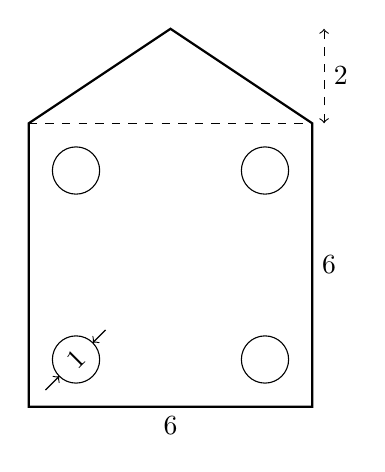
\begin{tikzpicture}[scale=0.6]
        \draw [thick]
        (0,0)--(0,6)--(3,8)--(6,6)--(6,0)--cycle;
        \draw [dashed] (0,6)--(6,6);
        \draw [dashed,<->] (6.25,6)--(6.25,8);
        \draw (1,1) circle[radius=0.5] node[rotate=45]{1};
        \draw [->] (45:0.5)--(45:0.9142);
        \draw [->] (45:2.3)--(45:1.9142);
        \draw (5,1) circle[radius=0.5];
        \draw (5,5) circle[radius=0.5];
        \draw (1,5) circle[radius=0.5];
        %\draw (0,8)++(0,-0.8)--++(0.8,0)--+(0,0.8);
        \node at (3,0)[below]{$6$};
        \node at (6,3)[right]{$6$};
        \node at (6.25,7)[right]{$2$};
      \end{tikzpicture} \vspace{1cm}
    \item Find the volume of the plate, to the \emph{nearest tenth of a cubic inch}. \vspace{2cm}
    \item Find the weight of the plate, to the \emph{nearest ounce}.
  \end{enumerate} \vspace{1.5cm}

\subsubsection*{Density and Price Reference Table}
\renewcommand{\arraystretch}{1.3}
\begin{tabular}{|l|r|r|}
    \hline
  Material & Density & Price\\
  \hline
  Steel & 0.282 lb./in.$^3$ & \$0.40/lb.\\
  \hline
  Brass & 0.307 lb./in.$^3$ & \$5.00/lb.\\
  \hline
  Aluminum & 0.096 lb./in.$^3$ & \$1.60/lb.\\
  \hline
  Titanium & 0.163 lb./in.$^3$ & \$26.00/lb.\\
  \hline
  Gold & 0.694 lb./in.$^3$ & \$1300/oz.\\
  \hline
  Plastic & 0.032 lb./in.$^3$ & \$0.70/oz.\\
  \hline
  Marble & 0.098 lb./in.$^3$ & \$3.00/oz.\\
  \hline
\end{tabular}


  \end{enumerate}
  \newpage
  \setcounter{page}{1}
\subsubsection*{11.1 Homework: Cross sections and 3-dimensional rotations}
 \begin{enumerate}
  \item A cube has a volume of 670 cubic inches. What is the length of its side, to the \emph{nearest hundredth of an inch}? \vspace{3cm}

  \item The Great Pyramid of Giza was constructed as a regular pyramid with a square base. It was built with an approximate volume of 2,592,276 cubic meters and a height of 1.46.5 meters. What was the length of one side of its base, to the \emph{nearest meter}? \vspace{5cm}

  \item A bakery sells hollow chocolate spheres. The larger diameter of each sphere is 4 cm. The thickness of the chocolate of each sphere is 0.5 cm. Determine and state , to the nearest tenth of a cubic centimeter, the amount of chocolate in each hollow sphere.\\[4.5cm]
  The bakery packages 8 of them into a box. If the density of the chocolate is 1.308 g/$\mathrm{cm}^3$, determine and state, to the nearest gram, the total mass of the chocolate in the box.

\newpage
\item A concrete ramp with a $4^\circ$ angle of elevation leads to a platform with a staircase stepping down from the opposite side, as shown below. The length of the platform is 3 feet, and each of the four steps has a rise of 7 inches and run of 10 inches. Find the length of the ramp $x$, to the \emph{nearest inch}.\\[0.25cm]
      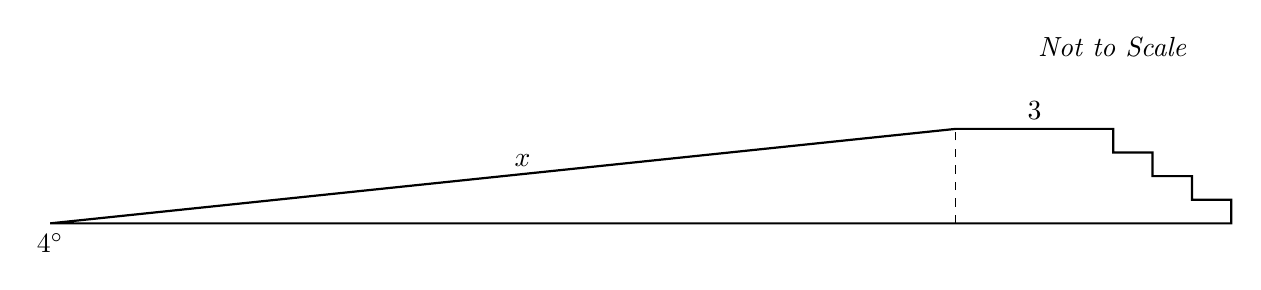
\begin{tikzpicture}[scale=0.5]
        \draw [thick] (7,0)--(30,2.4)--(34,2.4)--(34,1.8)--(35,1.8)--(35,1.2)--(36,1.2)--(36,0.6)--(37,0.6)--(37,0)--cycle;
        \draw [dashed] (30,0)--(30,2.4);
        %\draw (10,16)++(0,-0.8)--++(0.8,0)--+(0,0.8);
        \node at (32,2.4)[above]{$3$};
        \node at (7,0)[below]{$4^\circ$};
        \node at (19, 1.2)[above]{$x$};
        \node at (34, 4)[above]{\emph{Not to Scale}};
      \end{tikzpicture} \vspace{5cm}

\item A prescription medicine comes in capsule form. The capsule is in the shape of a cylinder with hemispherical ends, as shown in the rendering below. The capsule is 15 millimeters long by 8 millimeters across.
\begin{enumerate}
    \item Write down the radius $r$ of the capsule and the length of the cylindical portion $a$, shown in the diagram.\\
    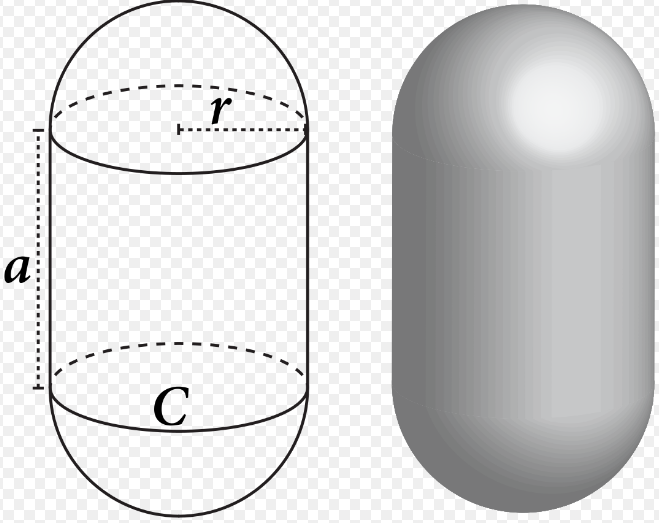
\includegraphics[width=0.3\textwidth]{capsule.png}\\
    \item Find the volume of the capsule to the \emph{nearest cubic millimeter}.
  \end{enumerate}

\end{enumerate}
\end{document}
